\newpage
%Nicht anfassen, so ist der Dokumentenaufbau
%\addtocontents{toc}{\protect\setcounter{tocdepth}{0}}
%\renewcommand{\appendixtocname}{Anhang}
%\addappheadtotoc % Überschrift 'Anhang' in TOC
%\renewcommand{\appendixpagename}{Anhang}
%\appendices
%\appendixpage
%\appendixtitleoff
\section*{Appendix}
\addcontentsline{toc}{section}{Appendix}
\setlength{\footskip}{35pt}

\begin{table}[!ht]
    \centering
    \begin{tabular}{lll}
    \hline
        \textbf{organism} & \textbf{\# metabolites} & \textbf{\# reactions} \\ \hline
        e\_coli\_core & 72 & 95 \\ \hline
        iAB\_RBC\_283 & 342 & 469 \\ \hline
        iIS312\_Amastigote & 606 & 519 \\ \hline
        iAF692 & 628 & 690 \\ \hline
        iSB619 & 655 & 743 \\ \hline
        iNF517 & 650 & 754 \\ \hline
        iHN637 & 698 & 785 \\ \hline
        iJB785 & 768 & 849 \\ \hline
        iNJ661 & 825 & 1025 \\ \hline
        iSynCJ816 & 928 & 1044 \\ \hline
        iJN746 & 907 & 1054 \\ \hline
        iJR904 & 761 & 1075 \\ \hline
        iEK1008 & 998 & 1226 \\ \hline
        iCN900 & 885 & 1229 \\ \hline
        iYO844 & 990 & 1250 \\ \hline
        iND750 & 1059 & 1266 \\ \hline
        iMM904 & 1226 & 1577 \\ \hline
        iRC1080 & 1706 & 2191 \\ \hline
        iAF1260 & 1668 & 2382 \\ \hline
        iSDY\_1059 & 1888 & 2539 \\ \hline
        STM\_v1\_0 & 1802 & 2545 \\ \hline
        iJO1366 & 1805 & 2583 \\ \hline
        iSbBS512\_1146 & 1910 & 2591 \\ \hline
        iS\_1188 & 1914 & 2619 \\ \hline
        iSFV\_1184 & 1917 & 2621 \\ \hline
        iSF\_1195 & 1917 & 2630 \\ \hline
        iSFxv\_1172 & 1918 & 2638 \\ \hline
        iML1515 & 1877 & 2712 \\ \hline
        iZ\_1308 & 1923 & 2721 \\ \hline
        iAPECO1\_1312 & 1942 & 2735 \\ \hline
        iECB\_1328 & 1951 & 2748 \\ \hline
        iETEC\_1333 & 1962 & 2756 \\ \hline
        iYS1720 & 2436 & 3357 \\ \hline
        iMM1415 & 2775 & 3726 \\ \hline
        RECON1 & 2766 & 3741 \\ \hline
        iLB1027\_lipid & 2172 & 4456 \\ \hline
        Recon3D & 5835 & 10600 \\ \hline
    \end{tabular}
    \caption{\label{Tab:big_model_size} Model size of used BiGG models.}
\end{table}

% \begin{table}[!ht]
%     \small
%     \centering
%     \begin{tabular}{|l|l|l|l|l|l|l|}
%     \hline
%     \multicolumn{1}{|c}{} & \multicolumn{3}{|c|}{ll-FBA} & \multicolumn{3}{c|}{ll-FBA (nullspace)}\\ \hline 
%     \textbf{organism} & \textbf{termination} & \textbf{o. v.} & \textbf{time (s)} & \textbf{termination} & \textbf{o. v.} & \textbf{time (s)} \\ \hline    
%         e\_coli\_core & OPTIMAL & 0.874 & 0 & OPTIMAL & 0.874 & 0 \\ \hline
%         iAB\_RBC\_283 & OPTIMAL & 2.936 & 0 & OPTIMAL & 2.936 & 2 \\ \hline
%         iIS312\_Amastigote & OPTIMAL & 25.339 & 0 & OPTIMAL & 25.339 & 0 \\ \hline
%         iAF692 & OPTIMAL & 0.027 & 3 & TIME\_LIMIT & 0.026 & 1800 \\ \hline
%         iSB619 & INFEASIBLE & NaN & 1 & TIME\_LIMIT & 0.027 & 1800 \\ \hline
%         iNF517 & OPTIMAL & 0.043 & 11 & OPTIMAL & 0.043 & 39 \\ \hline
%         iHN637 & OPTIMAL & 0.224 & 4 & OPTIMAL & 0.224 & 5 \\ \hline
%         iJB785 & OPTIMAL & 0.054 & 15 & OPTIMAL & 0.0 & 25 \\ \hline
%         iNJ661 & OPTIMAL & 0.053 & 181 & OPTIMAL & 0.053 & 227 \\ \hline
%         iSynCJ816 & OPTIMAL & 0.0 & 1 & INFEASIBLE & NaN & 34 \\ \hline
%         iJN746 & OPTIMAL & 1.4 & 332 & TIME\_LIMIT & NaN & 1800 \\ \hline
%         iJR904 & OPTIMAL & 0.922 & 93 & OPTIMAL & 0.922 & 163 \\ \hline
%         iEK1008 & OPTIMAL & 0.058 & 865 & OPTIMAL & 0.058 & 503 \\ \hline
%         iCN900 & OPTIMAL & 0.0 & 0 & OPTIMAL & 0.0 & 27 \\ \hline
%         iYO844 & TIME\_LIMIT & 0.115 & 1800 & TIME\_LIMIT & 0.0 & 1800 \\ \hline
%         iND750 & OPTIMAL & 0.0 & 8 & OPTIMAL & 0.0 & 151 \\ \hline
%         iMM904 & OPTIMAL & 0.288 & 1465 & TIME\_LIMIT & 0.0 & 1800 \\ \hline
%         iRC1080 & OPTIMAL & 0.0 & 373 & TIME\_LIMIT & NaN & 1800 \\ \hline
%         iAF1260 & TIME\_LIMIT & 0.69 & 1800 & TIME\_LIMIT & 0.0 & 1800 \\ \hline
%         iSDY\_1059 & TIME\_LIMIT & 0.92 & 1800 & TIME\_LIMIT & 0.0 & 1800 \\ \hline
%         STM\_v1\_0 & TIME\_LIMIT & 0.0 & 1800 & TIME\_LIMIT & 0.0 & 1800 \\ \hline
%         iJO1366 & TIME\_LIMIT & 0.939 & 1800 & TIME\_LIMIT & 0.0 & 1800 \\ \hline
%         iSbBS512\_1146 & TIME\_LIMIT & 0.0 & 1800 & TIME\_LIMIT & 0.0 & 1800 \\ \hline
%         iS\_1188 & TIME\_LIMIT & 0.73 & 1800 & TIME\_LIMIT & 0.0 & 1800 \\ \hline
%         iSFV\_1184 & OPTIMAL & 0.894 & 1241 & TIME\_LIMIT & 0.0 & 1800 \\ \hline
%         iSF\_1195 & TIME\_LIMIT & 0.915 & 1800 & TIME\_LIMIT & -0.0 & 1800 \\ \hline
%         iSFxv\_1172 & OPTIMAL & 0.894 & 966 & TIME\_LIMIT & 0.0 & 1800 \\ \hline
%         iML1515 & OPTIMAL & 0.877 & 1692 & TIME\_LIMIT & NaN & 1800 \\ \hline
%         iZ\_1308 & TIME\_LIMIT & 0.0 & 1800 & TIME\_LIMIT & 0.0 & 1800 \\ \hline
%         iAPECO1\_1312 & TIME\_LIMIT & 0.934 & 1800 & TIME\_LIMIT & 0.0 & 1800 \\ \hline
%         iECB\_1328 & TIME\_LIMIT & 0.0 & 1800 & TIME\_LIMIT & 0.0 & 1800 \\ \hline
%         iETEC\_1333 & TIME\_LIMIT & 0.0 & 1800 & TIME\_LIMIT & 0.0 & 1800 \\ \hline
%         iYS1720 & TIME\_LIMIT & 0.0 & 1800 & TIME\_LIMIT & NaN & 1800 \\ \hline
%         iMM1415 & OPTIMAL & 0.0 & 1550 & TIME\_LIMIT & NaN & 1800 \\ \hline
%         RECON1 & OPTIMAL & 0.0 & 83 & TIME\_LIMIT & NaN & 1800 \\ \hline
%         iLB1027\_lipid & TIME\_LIMIT & 0.0 & 1800 & TIME\_LIMIT & NaN & 1800 \\ \hline
%         Recon3D & TIME\_LIMIT & NaN & 1800 & TIME\_LIMIT & NaN & 1800 \\ \hline
%     \end{tabular}
%     \caption{\label{Tab:ll_fba_comparison} Results of using the nullspace formulation vs the reformulation.}
% \end{table}

% \begin{table}[!ht]
%     \small
%     \centering
%     \begin{tabular}{|l|l|l|l|l|l|l|}
%     \hline
%     \multicolumn{1}{|c}{} & \multicolumn{2}{|c|}{ll-FBA} & \multicolumn{2}{|c|}{CB (indicator)} & \multicolumn{2}{c|}{CB (big M)}\\ \hline 
%     organism & termination & time & termination & time & termination & time \\ \hline
%         iAF692 & OPTIMAL & 3 & OPTIMAL & 16.0 & OPTIMAL & 7.0 \\ \hline
%         iSB619 & INFEASIBLE & 1 & OPTIMAL & 15.0 & OPTIMAL & 6.0 \\ \hline
%         iNF517 & OPTIMAL & 11 & OPTIMAL & 29.0 & OPTIMAL & 12.0 \\ \hline
%         iHN637 & OPTIMAL & 4 & OPTIMAL & 11.0 & OPTIMAL & 7.0 \\ \hline
%         iJB785 & OPTIMAL & 15 & OPTIMAL & 14.0 & OPTIMAL & 7.0 \\ \hline
%         iNJ661 & OPTIMAL & 181 & OPTIMAL & 61.0 & OPTIMAL & 9.0 \\ \hline
%         iSynCJ816 & OPTIMAL & 1 & ERROR & NaN & ERROR & NaN \\ \hline
%         iJN746 & OPTIMAL & 332 & OPTIMAL & 41.0 & OPTIMAL & 237.0 \\ \hline
%         iJR904 & OPTIMAL & 93 & OPTIMAL & 21.0 & OPTIMAL & 12.0 \\ \hline
%         iEK1008 & OPTIMAL & 865 & OPTIMAL & 20.0 & OPTIMAL & 9.0 \\ \hline
%         iCN900 & OPTIMAL & 0 & OPTIMAL & 11.0 & OPTIMAL & 6.0 \\ \hline
%         iYO844 & TIME\_LIMIT & 1800 & OPTIMAL & 26.0 & OPTIMAL & 8.0 \\ \hline
%         iND750 & OPTIMAL & 8 & OPTIMAL & 46.0 & OPTIMAL & 10.0 \\ \hline
%         iMM904 & OPTIMAL & 1465 & OPTIMAL & 154.0 & OPTIMAL & 24.0 \\ \hline
%         iRC1080 & OPTIMAL & 373 & ERROR & 1800.0 & ERROR & NaN \\ \hline
%         iAF1260 & TIME\_LIMIT & 1800 & OPTIMAL & 166.0 & OPTIMAL & 39.0 \\ \hline
%         iSDY\_1059 & TIME\_LIMIT & 1800 & OPTIMAL & 273.0 & OPTIMAL & 46.0 \\ \hline
%         STM\_v1\_0 & TIME\_LIMIT & 1800 & OPTIMAL & 105.0 & OPTIMAL & 23.0 \\ \hline
%         iJO1366 & TIME\_LIMIT & 1800 & OPTIMAL & 286.0 & OPTIMAL & 52.0 \\ \hline
%         iSbBS512\_1146 & TIME\_LIMIT & 1800 & OPTIMAL & 360.0 & OPTIMAL & 118.0 \\ \hline
%         iS\_1188 & TIME\_LIMIT & 1800 & OPTIMAL & 311.0 & OPTIMAL & 52.0 \\ \hline
%         iSFV\_1184 & OPTIMAL & 1241 & OPTIMAL & 442.0 & OPTIMAL & 85.0 \\ \hline
%         iSF\_1195 & TIME\_LIMIT & 1800 & OPTIMAL & 452.0 & OPTIMAL & 43.0 \\ \hline
%         iSFxv\_1172 & OPTIMAL & 966 & OPTIMAL & 301.0 & OPTIMAL & 53.0 \\ \hline
%         iML1515 & OPTIMAL & 1692 & OPTIMAL & 188.0 & OPTIMAL & 33.0 \\ \hline
%         iZ\_1308 & TIME\_LIMIT & 1800 & OPTIMAL & 536.0 & OPTIMAL & 83.0 \\ \hline
%         iAPECO1\_1312 & TIME\_LIMIT & 1800 & OPTIMAL & 954.0 & OPTIMAL & 107.0 \\ \hline
%         iECB\_1328 & TIME\_LIMIT & 1800 & OPTIMAL & 486.0 & OPTIMAL & 80.0 \\ \hline
%         iETEC\_1333 & TIME\_LIMIT & 1800 & OPTIMAL & 544.0 & OPTIMAL & 88.0 \\ \hline
%         iYS1720 & TIME\_LIMIT & 1800 & OPTIMAL & 463.0 & OPTIMAL & 94.0 \\ \hline
%         iMM1415 & OPTIMAL & 1550 & OPTIMAL & 1800.0 & OPTIMAL & 110.0 \\ \hline
%         RECON1 & OPTIMAL & 83 & OPTIMAL & 1800.0 & OPTIMAL & 297.0 \\ \hline
%         iLB1027\_lipid & TIME\_LIMIT & 1800 & TIME\_LIMIT & 1800.0 & INFEASIBLE & 1800.0 \\ \hline
%         Recon3D & TIME\_LIMIT & 1800 & TIME\_LIMIT & 1800.0 & INFEASIBLE & 1800.0 \\ \hline
%     \end{tabular}
%     \caption{\label{Tab:cb_vs_llfba} Results of using ll-FBA vs CB with indicator and CB with big M formulation.}
% \end{table}

% llfba_vs_nullspace 
\begin{table}[!ht]
    \small
    \centering
    \begin{tabular}{|l|l|l|l|l|l|l|}
    \hline
        \multicolumn{1}{|c}{} & \multicolumn{3}{|c|}{ll-FBA} & \multicolumn{3}{c|}{ll-FBA (nullspace)}\\ \hline 
        organism & termination & time & o. v. & termination & time & o. v. \\ \hline
        e\_coli\_core & OPTIMAL & 0 & 0.874 & OPTIMAL & 0 & 0.874 \\ \hline
        iAB\_RBC\_283 & OPTIMAL & 0 & 2.936 & OPTIMAL & 2 & 2.936 \\ \hline
        iIS312\_Amastigote & OPTIMAL & 0 & 25.339 & OPTIMAL & 0 & 25.339 \\ \hline
        iAF692 & OPTIMAL & 3 & 0.027 & TIME\_LIMIT & 1800 & 0.026 \\ \hline
        iSB619 & INFEASIBLE & 1 & NaN & TIME\_LIMIT & 1800 & 0.027 \\ \hline
        iNF517 & OPTIMAL & 11 & 0.043 & OPTIMAL & 39 & 0.043 \\ \hline
        iHN637 & OPTIMAL & 4 & 0.224 & OPTIMAL & 5 & 0.224 \\ \hline
        iJB785 & OPTIMAL & 15 & 0.054 & OPTIMAL & 25 & 0.0 \\ \hline
        iNJ661 & OPTIMAL & 181 & 0.053 & OPTIMAL & 227 & 0.053 \\ \hline
        iSynCJ816 & OPTIMAL & 1 & 0.0 & INFEASIBLE & 34 & NaN \\ \hline
        iJN746 & OPTIMAL & 332 & 1.4 & TIME\_LIMIT & 1800 & NaN \\ \hline
        iJR904 & OPTIMAL & 93 & 0.922 & OPTIMAL & 163 & 0.922 \\ \hline
        iEK1008 & OPTIMAL & 865 & 0.058 & OPTIMAL & 503 & 0.058 \\ \hline
        iCN900 & OPTIMAL & 0 & 0.0 & OPTIMAL & 27 & 0.0 \\ \hline
        iYO844 & TIME\_LIMIT & 1800 & 0.115 & TIME\_LIMIT & 1800 & 0.0 \\ \hline
        iND750 & OPTIMAL & 8 & 0.0 & OPTIMAL & 151 & 0.0 \\ \hline
        iMM904 & OPTIMAL & 1465 & 0.288 & TIME\_LIMIT & 1800 & 0.0 \\ \hline
        iRC1080 & OPTIMAL & 373 & 0.0 & TIME\_LIMIT & 1800 & NaN \\ \hline
        iAF1260 & TIME\_LIMIT & 1800 & 0.69 & TIME\_LIMIT & 1800 & 0.0 \\ \hline
        iSDY\_1059 & TIME\_LIMIT & 1800 & 0.92 & TIME\_LIMIT & 1800 & 0.0 \\ \hline
        STM\_v1\_0 & TIME\_LIMIT & 1800 & 0.0 & TIME\_LIMIT & 1800 & 0.0 \\ \hline
        iJO1366 & TIME\_LIMIT & 1800 & 0.939 & TIME\_LIMIT & 1800 & 0.0 \\ \hline
        iSbBS512\_1146 & TIME\_LIMIT & 1800 & 0.0 & TIME\_LIMIT & 1800 & 0.0 \\ \hline
        iS\_1188 & TIME\_LIMIT & 1800 & 0.73 & TIME\_LIMIT & 1800 & 0.0 \\ \hline
        iSFV\_1184 & OPTIMAL & 1241 & 0.894 & TIME\_LIMIT & 1800 & 0.0 \\ \hline
        iSF\_1195 & TIME\_LIMIT & 1800 & 0.915 & TIME\_LIMIT & 1800 & -0.0 \\ \hline
        iSFxv\_1172 & OPTIMAL & 966 & 0.894 & TIME\_LIMIT & 1800 & 0.0 \\ \hline
        iML1515 & OPTIMAL & 1692 & 0.877 & TIME\_LIMIT & 1800 & NaN \\ \hline
        iZ\_1308 & TIME\_LIMIT & 1800 & 0.0 & TIME\_LIMIT & 1800 & 0.0 \\ \hline
        iAPECO1\_1312 & TIME\_LIMIT & 1800 & 0.934 & TIME\_LIMIT & 1800 & 0.0 \\ \hline
        iECB\_1328 & TIME\_LIMIT & 1800 & 0.0 & TIME\_LIMIT & 1800 & 0.0 \\ \hline
        iETEC\_1333 & TIME\_LIMIT & 1800 & 0.0 & TIME\_LIMIT & 1800 & 0.0 \\ \hline
        iYS1720 & TIME\_LIMIT & 1800 & 0.0 & TIME\_LIMIT & 1800 & NaN \\ \hline
        iMM1415 & OPTIMAL & 1550 & 0.0 & TIME\_LIMIT & 1800 & NaN \\ \hline
        RECON1 & OPTIMAL & 83 & 0.0 & TIME\_LIMIT & 1800 & NaN \\ \hline
        iLB1027\_lipid & TIME\_LIMIT & 1800 & 0.0 & TIME\_LIMIT & 1800 & NaN \\ \hline
        Recon3D & TIME\_LIMIT & 1800 & NaN & TIME\_LIMIT & 1800 & NaN \\ \hline
    \end{tabular}
    \caption{\label{Tab:ll_fba_comparison} Results of using the nullspace formulation vs the reformulation.}
\end{table}


% cb_vs_nullspace
\begin{table}[!ht]
    \small
    \centering
    \begin{tabular}{|l|l|l|l|l|l|l|}
    \hline
        \multicolumn{1}{|c}{} & \multicolumn{2}{|c|}{ll-FBA} & \multicolumn{2}{|c|}{CB (indicator)} & \multicolumn{2}{c|}{CB (big M)}\\ \hline 
        organism & termination & time & termination & time & termination & time \\ \hline
        e\_coli\_core & OPTIMAL & 0 & OPTIMAL & 9 & OPTIMAL & 5 \\ \hline
        iAB\_RBC\_283 & OPTIMAL & 0 & OPTIMAL & 11 & OPTIMAL & 5 \\ \hline
        iIS312\_Amastigote & OPTIMAL & 0 & OPTIMAL & 10 & OPTIMAL & 6 \\ \hline
        iAF692 & OPTIMAL & 3 & OPTIMAL & 16 & OPTIMAL & 7 \\ \hline
        iSB619 & INFEASIBLE & 1 & OPTIMAL & 15 & OPTIMAL & 6 \\ \hline
        iNF517 & OPTIMAL & 11 & OPTIMAL & 29 & OPTIMAL & 12 \\ \hline
        iHN637 & OPTIMAL & 4 & OPTIMAL & 11 & OPTIMAL & 7 \\ \hline
        iJB785 & OPTIMAL & 15 & OPTIMAL & 14 & OPTIMAL & 7 \\ \hline
        iNJ661 & OPTIMAL & 181 & OPTIMAL & 61 & OPTIMAL & 9 \\ \hline
        iSynCJ816 & OPTIMAL & 1 & ERROR & ~ & ERROR & ~ \\ \hline
        iJN746 & OPTIMAL & 332 & OPTIMAL & 41 & OPTIMAL & 237 \\ \hline
        iJR904 & OPTIMAL & 93 & OPTIMAL & 21 & OPTIMAL & 12 \\ \hline
        iEK1008 & OPTIMAL & 865 & OPTIMAL & 20 & OPTIMAL & 9 \\ \hline
        iCN900 & OPTIMAL & 0 & OPTIMAL & 11 & OPTIMAL & 6 \\ \hline
        iYO844 & TIME\_LIMIT & 1800 & OPTIMAL & 26 & OPTIMAL & 8 \\ \hline
        iND750 & OPTIMAL & 8 & OPTIMAL & 46 & OPTIMAL & 10 \\ \hline
        iMM904 & OPTIMAL & 1465 & OPTIMAL & 154 & OPTIMAL & 24 \\ \hline
        iRC1080 & OPTIMAL & 373 & TIME\_LIMIT & 1800 & ERROR & ~ \\ \hline
        iAF1260 & TIME\_LIMIT & 1800 & OPTIMAL & 166 & OPTIMAL & 39 \\ \hline
        iSDY\_1059 & TIME\_LIMIT & 1800 & OPTIMAL & 273 & OPTIMAL & 46 \\ \hline
        STM\_v1\_0 & TIME\_LIMIT & 1800 & OPTIMAL & 105 & OPTIMAL & 23 \\ \hline
        iJO1366 & TIME\_LIMIT & 1800 & OPTIMAL & 286 & OPTIMAL & 52 \\ \hline
        iSbBS512\_1146 & TIME\_LIMIT & 1800 & OPTIMAL & 360 & OPTIMAL & 118 \\ \hline
        iS\_1188 & TIME\_LIMIT & 1800 & OPTIMAL & 311 & OPTIMAL & 52 \\ \hline
        iSFV\_1184 & OPTIMAL & 1241 & OPTIMAL & 442 & OPTIMAL & 85 \\ \hline
        iSF\_1195 & TIME\_LIMIT & 1800 & OPTIMAL & 452 & OPTIMAL & 43 \\ \hline
        iSFxv\_1172 & OPTIMAL & 966 & OPTIMAL & 301 & OPTIMAL & 53 \\ \hline
        iML1515 & OPTIMAL & 1692 & OPTIMAL & 188 & OPTIMAL & 33 \\ \hline
        iZ\_1308 & TIME\_LIMIT & 1800 & OPTIMAL & 536 & OPTIMAL & 83 \\ \hline
        iAPECO1\_1312 & TIME\_LIMIT & 1800 & OPTIMAL & 954 & OPTIMAL & 107 \\ \hline
        iECB\_1328 & TIME\_LIMIT & 1800 & OPTIMAL & 486 & OPTIMAL & 80 \\ \hline
        iETEC\_1333 & TIME\_LIMIT & 1800 & OPTIMAL & 544 & OPTIMAL & 88 \\ \hline
        iYS1720 & TIME\_LIMIT & 1800 & OPTIMAL & 463 & OPTIMAL & 94 \\ \hline
        iMM1415 & OPTIMAL & 1550 & TIME\_LIMIT & 1800 & OPTIMAL & 110 \\ \hline
        RECON1 & OPTIMAL & 83 & TIME\_LIMIT & 1800 & OPTIMAL & 297 \\ \hline
        iLB1027\_lipid & TIME\_LIMIT & 1800 & TIME\_LIMIT & 1800 & TIME\_LIMIT & 1800 \\ \hline
        Recon3D & TIME\_LIMIT & 1800 & TIME\_LIMIT & 1800 & TIME\_LIMIT & 1800 \\ \hline
    \end{tabular}
    \caption{\label{Tab:cb_vs_llfba} Results of using ll-FBA vs CB with indicator and CB with big M formulation.}
\end{table}

% no_good_cuts_big_m
\begin{table}[!ht]
    \small
    \centering
    \begin{tabular}{|l|l|l|l|l|l|l|}
    \hline
        \multicolumn{1}{|c}{} & \multicolumn{3}{|c|}{CB (big M)} & \multicolumn{3}{c|}{No Good Cuts (big M)}\\ \hline 
        organism & termination & time & o. v. & termination & time & o. v. \\ \hline
        e\_coli\_core & OPTIMAL & 5 & 0.874 & OPTIMAL & 6 & 0.874 \\ \hline
        iAB\_RBC\_283 & OPTIMAL & 5 & 2.936 & TIME\_LIMIT & 1800 & 2.936 \\ \hline
        iIS312\_Amastigote & OPTIMAL & 6 & 25.339 & TIME\_LIMIT & 1800 & 25.339 \\ \hline
        iAF692 & OPTIMAL & 7 & 0.013 & ERROR & ~ & NaN \\ \hline
        iSB619 & OPTIMAL & 6 & 0.158 & TIME\_LIMIT & 1800 & 0.158 \\ \hline
        iNF517 & OPTIMAL & 12 & 0.043 & TIME\_LIMIT & 1800 & 0.043 \\ \hline
        iHN637 & OPTIMAL & 7 & 0.224 & TIME\_LIMIT & 1800 & 0.224 \\ \hline
        iJB785 & OPTIMAL & 7 & 0.054 & OPTIMAL & 9 & 0.0 \\ \hline
        iNJ661 & OPTIMAL & 9 & 0.052 & TIME\_LIMIT & 1800 & 0.0 \\ \hline
        iSynCJ816 & ERROR & ~ & NaN & TIME\_LIMIT & 1800 & 0.0 \\ \hline
        iJN746 & OPTIMAL & 237 & 1.4 & ERROR & ~ & NaN \\ \hline
        iJR904 & OPTIMAL & 12 & 0.922 & TIME\_LIMIT & 1800 & 0.922 \\ \hline
        iEK1008 & OPTIMAL & 9 & 0.058 & TIME\_LIMIT & 1800 & 0.058 \\ \hline
        iCN900 & OPTIMAL & 6 & 0.0 & TIME\_LIMIT & 1800 & 0.0 \\ \hline
        iYO844 & OPTIMAL & 8 & 0.118 & TIME\_LIMIT & 1800 & 0.118 \\ \hline
        iND750 & OPTIMAL & 10 & 0.0 & OPTIMAL & 6 & 0.0 \\ \hline
        iMM904 & OPTIMAL & 24 & 0.287 & TIME\_LIMIT & 1800 & 0.288 \\ \hline
        iRC1080 & ERROR & ~ & NaN & TIME\_LIMIT & 1800 & 0.0 \\ \hline
        iAF1260 & OPTIMAL & 39 & 0.737 & TIME\_LIMIT & 1800 & 0.722 \\ \hline
        iSDY\_1059 & OPTIMAL & 46 & 0.938 & TIME\_LIMIT & 1800 & 0.938 \\ \hline
        STM\_v1\_0 & OPTIMAL & 23 & 0.478 & TIME\_LIMIT & 1800 & 0.478 \\ \hline
        iJO1366 & OPTIMAL & 52 & 0.982 & TIME\_LIMIT & 1800 & 0.982 \\ \hline
        iSbBS512\_1146 & OPTIMAL & 118 & 0.983 & ERROR & ~ & NaN \\ \hline
        iS\_1188 & OPTIMAL & 52 & 0.857 & TIME\_LIMIT & 1800 & 0.857 \\ \hline
        iSFV\_1184 & OPTIMAL & 85 & 0.894 & TIME\_LIMIT & 1800 & 0.894 \\ \hline
        iSF\_1195 & OPTIMAL & 43 & 0.915 & TIME\_LIMIT & 1800 & 0.915 \\ \hline
        iSFxv\_1172 & OPTIMAL & 53 & 0.894 & TIME\_LIMIT & 1800 & 0.894 \\ \hline
        iML1515 & OPTIMAL & 33 & 0.877 & TIME\_LIMIT & 1800 & 0.877 \\ \hline
        iZ\_1308 & OPTIMAL & 83 & 0.982 & TIME\_LIMIT & 1800 & 0.982 \\ \hline
        iAPECO1\_1312 & OPTIMAL & 107 & 0.982 & TIME\_LIMIT & 1800 & 0.982 \\ \hline
        iECB\_1328 & OPTIMAL & 80 & 0.982 & TIME\_LIMIT & 1800 & 0.982 \\ \hline
        iETEC\_1333 & OPTIMAL & 88 & 0.982 & TIME\_LIMIT & 1800 & 0.982 \\ \hline
        iYS1720 & OPTIMAL & 94 & 0.488 & TIME\_LIMIT & 1800 & 0.488 \\ \hline
        iMM1415 & OPTIMAL & 110 & 0.0 & TIME\_LIMIT & 1800 & 0.0 \\ \hline
        RECON1 & OPTIMAL & 297 & 0.0 & TIME\_LIMIT & 1800 & 0.0 \\ \hline
        iLB1027\_lipid & TIME\_LIMIT & 1800 & 0.36 & TIME\_LIMIT & 1800 & 0.36 \\ \hline
        Recon3D & TIME\_LIMIT & 1800 & 755.003 & TIME\_LIMIT & 1800 & 755.003 \\ \hline
    \end{tabular}
    \caption{\label{Tab:cb_vs_ngc_big_m} Results of using no good cuts vs CB with big M formulation.}
\end{table}

% no_good_cuts_indicator
\begin{table}[!ht]
    \centering
    \begin{tabular}{|l|l|l|l|l|l|l|}
    \hline
        \multicolumn{1}{|c}{} & \multicolumn{3}{|c|}{CB (indicator)} & \multicolumn{3}{c|}{No Good Cuts (indicator)}\\ \hline 
        organism & termination & time & o. v. & termination & time & o. v. \\ \hline
        e\_coli\_core & OPTIMAL & 9 & 0.874 & TIME\_LIMIT & 1800 & 0.874 \\ \hline
        iAB\_RBC\_283 & OPTIMAL & 11 & 2.936 & TIME\_LIMIT & 1800 & 2.936 \\ \hline
        iIS312\_Amastigote & OPTIMAL & 10 & 25.339 & OPTIMAL & 12 & 25.339 \\ \hline
        iAF692 & OPTIMAL & 16 & 0.027 & TIME\_LIMIT & 1800 & 0.027 \\ \hline
        iSB619 & OPTIMAL & 15 & 0.158 & TIME\_LIMIT & 1800 & 0.158 \\ \hline
        iNF517 & OPTIMAL & 29 & 0.043 & TIME\_LIMIT & 1800 & 0.043 \\ \hline
        iHN637 & OPTIMAL & 11 & 0.224 & OPTIMAL & 613 & 0.224 \\ \hline
        iJB785 & OPTIMAL & 14 & 0.054 & OPTIMAL & 11 & 0.054 \\ \hline
        iNJ661 & OPTIMAL & 61 & 0.053 & TIME\_LIMIT & 1800 & 0.053 \\ \hline
        iSynCJ816 & ERROR & ~ & NaN & TIME\_LIMIT & 1800 & 0.0 \\ \hline
        iJN746 & OPTIMAL & 41 & 1.4 & TIME\_LIMIT & 1800 & 1.4 \\ \hline
        iJR904 & OPTIMAL & 21 & 0.922 & TIME\_LIMIT & 1800 & 0.922 \\ \hline
        iEK1008 & OPTIMAL & 20 & 0.058 & TIME\_LIMIT & 1800 & 0.058 \\ \hline
        iCN900 & OPTIMAL & 11 & 0.0 & TIME\_LIMIT & 1800 & 0.0 \\ \hline
        iYO844 & OPTIMAL & 26 & 0.118 & TIME\_LIMIT & 1800 & 0.118 \\ \hline
        iND750 & OPTIMAL & 46 & 0.097 & TIME\_LIMIT & 1800 & 0.097 \\ \hline
        iMM904 & OPTIMAL & 154 & 0.288 & TIME\_LIMIT & 1800 & 0.288 \\ \hline
        iRC1080 & TIME\_LIMIT & 1800 & 0.0 & TIME\_LIMIT & 1800 & 0.0 \\ \hline
        iAF1260 & OPTIMAL & 166 & 0.737 & TIME\_LIMIT & 1800 & 0.737 \\ \hline
        iSDY\_1059 & OPTIMAL & 273 & 0.938 & TIME\_LIMIT & 1800 & 0.938 \\ \hline
        STM\_v1\_0 & OPTIMAL & 105 & 0.478 & TIME\_LIMIT & 1800 & 0.478 \\ \hline
        iJO1366 & OPTIMAL & 286 & 0.982 & TIME\_LIMIT & 1800 & 0.982 \\ \hline
        iSbBS512\_1146 & OPTIMAL & 360 & 0.983 & TIME\_LIMIT & 1800 & 0.983 \\ \hline
        iS\_1188 & OPTIMAL & 311 & 0.857 & TIME\_LIMIT & 1800 & 0.857 \\ \hline
        iSFV\_1184 & OPTIMAL & 442 & 0.894 & TIME\_LIMIT & 1800 & 0.894 \\ \hline
        iSF\_1195 & OPTIMAL & 452 & 0.915 & TIME\_LIMIT & 1800 & 0.915 \\ \hline
        iSFxv\_1172 & OPTIMAL & 301 & 0.894 & TIME\_LIMIT & 1800 & 0.894 \\ \hline
        iML1515 & OPTIMAL & 188 & 0.877 & TIME\_LIMIT & 1800 & 0.877 \\ \hline
        iZ\_1308 & OPTIMAL & 536 & 0.982 & TIME\_LIMIT & 1800 & 0.982 \\ \hline
        iAPECO1\_1312 & OPTIMAL & 954 & 0.982 & TIME\_LIMIT & 1800 & 0.982 \\ \hline
        iECB\_1328 & OPTIMAL & 486 & 0.982 & TIME\_LIMIT & 1800 & 0.982 \\ \hline
        iETEC\_1333 & OPTIMAL & 544 & 0.982 & TIME\_LIMIT & 1800 & 0.982 \\ \hline
        iYS1720 & OPTIMAL & 463 & 0.488 & TIME\_LIMIT & 1800 & 0.488 \\ \hline
        iMM1415 & TIME\_LIMIT & 1800 & 0.0 & TIME\_LIMIT & 1800 & 0.0 \\ \hline
        RECON1 & TIME\_LIMIT & 1800 & 0.0 & TIME\_LIMIT & 1800 & 0.0 \\ \hline
        iLB1027\_lipid & TIME\_LIMIT & 1800 & 0.36 & TIME\_LIMIT & 1800 & 0.36 \\ \hline
        Recon3D & TIME\_LIMIT & 1800 & 190.883 & TIME\_LIMIT & 1800 & 190.883 \\ \hline
    \end{tabular}
    \caption{\label{Tab:cb_vs_ngc_indicator} Results of using no good cuts vs CB with indicator constraints.}
\end{table}

% multiple_mis_big_m
\begin{table}[!ht]
    \small
    \centering
    \begin{tabular}{|l|l|l|l|l|l|l|l|l|}
    \hline
        \multicolumn{1}{|c}{} & \multicolumn{2}{|c|}{CB (big M) MIS 5\%} & \multicolumn{2}{|c|}{CB (big M) MIS 10\%} & \multicolumn{2}{|c|}{CB (big M) MIS 20\%} & \multicolumn{2}{|c|}{CB (big M) MIS 30\%} \\ \hline
        organism & termination & time & termination & time & termination & time & termination & time \\ \hline
        e\_coli\_core & OPTIMAL & 5 & OPTIMAL & 6 & OPTIMAL & 5 & OPTIMAL & 5 \\ \hline
        iAB\_RBC\_283 & OPTIMAL & 6 & OPTIMAL & 5 & OPTIMAL & 6 & OPTIMAL & 6 \\ \hline
        iIS312\_Amastigote & OPTIMAL & 6 & OPTIMAL & 6 & OPTIMAL & 6 & OPTIMAL & 7 \\ \hline
        iAF692 & OPTIMAL & 6 & OPTIMAL & 7 & OPTIMAL & 12 & OPTIMAL & 16 \\ \hline
        iSB619 & OPTIMAL & 6 & OPTIMAL & 9 & OPTIMAL & 8 & OPTIMAL & 13 \\ \hline
        iNF517 & OPTIMAL & 6 & OPTIMAL & 6 & OPTIMAL & 6 & OPTIMAL & 7 \\ \hline
        iHN637 & OPTIMAL & 6 & OPTIMAL & 7 & OPTIMAL & 9 & OPTIMAL & 8 \\ \hline
        iJB785 & OPTIMAL & 6 & OPTIMAL & 7 & OPTIMAL & 8 & OPTIMAL & 7 \\ \hline
        iNJ661 & OPTIMAL & 22 & OPTIMAL & 23 & OPTIMAL & 41 & OPTIMAL & 41 \\ \hline
        iSynCJ816 & ERROR & ~ & ERROR & ~ & ERROR & ~ & ERROR & ~ \\ \hline
        iJN746 & OPTIMAL & 128 & OPTIMAL & 84 & OPTIMAL & 192 & OPTIMAL & 136 \\ \hline
        iJR904 & OPTIMAL & 9 & OPTIMAL & 9 & OPTIMAL & 78 & OPTIMAL & 14 \\ \hline
        iEK1008 & OPTIMAL & 10 & OPTIMAL & 9 & OPTIMAL & 21 & OPTIMAL & 10 \\ \hline
        iCN900 & OPTIMAL & 6 & OPTIMAL & 9 & OPTIMAL & 10 & OPTIMAL & 25 \\ \hline
        iYO844 & OPTIMAL & 9 & OPTIMAL & 8 & OPTIMAL & 10 & OPTIMAL & 49 \\ \hline
        iND750 & OPTIMAL & 10 & OPTIMAL & 19 & OPTIMAL & 15 & OPTIMAL & 43 \\ \hline
        iMM904 & OPTIMAL & 33 & OPTIMAL & 70 & OPTIMAL & 146 & OPTIMAL & 183 \\ \hline
        iRC1080 & ERROR & ~ & OPTIMAL & 412 & OPTIMAL & 290 & ERROR & ~ \\ \hline
        iAF1260 & OPTIMAL & 15 & OPTIMAL & 42 & OPTIMAL & 89 & OPTIMAL & 1712 \\ \hline
        iSDY\_1059 & TIME\_LIMIT & 1800 & TIME\_LIMIT & 1800 & TIME\_LIMIT & 1800 & OPTIMAL & 199 \\ \hline
        STM\_v1\_0 & OPTIMAL & 52 & TIME\_LIMIT & 1800 & OPTIMAL & 934 & OPTIMAL & 1565 \\ \hline
        iJO1366 & OPTIMAL & 30 & OPTIMAL & 56 & TIME\_LIMIT & 1800 & TIME\_LIMIT & 1800 \\ \hline
        iSbBS512\_1146 & ERROR & ~ & ERROR & ~ & ERROR & ~ & ERROR & ~ \\ \hline
        iS\_1188 & OPTIMAL & 21 & OPTIMAL & 43 & TIME\_LIMIT & 1800 & TIME\_LIMIT & 1800 \\ \hline
        iSFV\_1184 & TIME\_LIMIT & 1800 & OPTIMAL & 60 & OPTIMAL & 42 & TIME\_LIMIT & 1800 \\ \hline
        iSF\_1195 & TIME\_LIMIT & 1800 & TIME\_LIMIT & 1800 & TIME\_LIMIT & 1800 & OPTIMAL & 1654 \\ \hline
        iSFxv\_1172 & TIME\_LIMIT & 1800 & OPTIMAL & 1800 & TIME\_LIMIT & 1800 & TIME\_LIMIT & 1800 \\ \hline
        iML1515 & TIME\_LIMIT & 1800 & TIME\_LIMIT & 1800 & TIME\_LIMIT & 1800 & TIME\_LIMIT & 1800 \\ \hline
        iZ\_1308 & OPTIMAL & 69 & TIME\_LIMIT & 1800 & TIME\_LIMIT & 1800 & TIME\_LIMIT & 1800 \\ \hline
        iAPECO1\_1312 & OPTIMAL & 97 & OPTIMAL & 1559 & TIME\_LIMIT & 1800 & TIME\_LIMIT & 1800 \\ \hline
        iECB\_1328 & OPTIMAL & 68 & TIME\_LIMIT & 1800 & TIME\_LIMIT & 1800 & TIME\_LIMIT & 1800 \\ \hline
        iETEC\_1333 & OPTIMAL & 35 & TIME\_LIMIT & 1800 & TIME\_LIMIT & 1800 & TIME\_LIMIT & 1800 \\ \hline
        iYS1720 & OPTIMAL & 203 & OPTIMAL & 1155 & TIME\_LIMIT & 1800 & TIME\_LIMIT & 1800 \\ \hline
        iMM1415 & OPTIMAL & 1769 & OPTIMAL & 1380 & TIME\_LIMIT & 1800 & TIME\_LIMIT & 1800 \\ \hline
        RECON1 & TIME\_LIMIT & 1800 & TIME\_LIMIT & 1800 & TIME\_LIMIT & 1800 & TIME\_LIMIT & 1800 \\ \hline
        iLB1027\_lipid & TIME\_LIMIT & 1800 & TIME\_LIMIT & 1800 & TIME\_LIMIT & 1800 & TIME\_LIMIT & 1800 \\ \hline
        Recon3D & TIME\_LIMIT & 1800 & TIME\_LIMIT & 1800 & TIME\_LIMIT & 1800 & TIME\_LIMIT & 1800 \\ \hline
    \end{tabular}
    \caption{\label{Tab:multiple_mis_big_m} Results of searching multiple MIS in CB with big M formulation.}
\end{table}

% multiple_mis_indicator
\begin{table}[!ht]
    \small
    \centering
    \begin{tabular}{|l|l|l|l|l|l|l|l|l|}
    \hline
        \multicolumn{1}{|c}{} & \multicolumn{2}{|c|}{CB (indicator) MIS 5\%} & \multicolumn{2}{|c|}{CB (indicator) MIS 10\%} & \multicolumn{2}{|c|}{CB (indicator) MIS 20\%} & \multicolumn{2}{|c|}{CB (indicator) MIS 30\%} \\ \hline
        organism & termination\_cb\_mis\_5 & time\_cb\_mis\_5 & termination\_cb\_mis\_10 & time\_cb\_mis\_10 & termination\_cb\_mis\_20 & time\_cb\_mis\_20 & termination\_cb\_mis\_30 & time\_cb\_mis\_30 \\ \hline
        e\_coli\_core & OPTIMAL & 9 & OPTIMAL & 9 & OPTIMAL & 9 & OPTIMAL & 9 \\ \hline
        iAB\_RBC\_283 & OPTIMAL & 10 & OPTIMAL & 10 & OPTIMAL & 10 & OPTIMAL & 10 \\ \hline
        iIS312\_Amastigote & OPTIMAL & 10 & OPTIMAL & 10 & OPTIMAL & 11 & OPTIMAL & 10 \\ \hline
        iAF692 & OPTIMAL & 14 & OPTIMAL & 14 & OPTIMAL & 14 & OPTIMAL & 13 \\ \hline
        iSB619 & OPTIMAL & 11 & OPTIMAL & 12 & OPTIMAL & 22 & OPTIMAL & 11 \\ \hline
        iNF517 & OPTIMAL & 12 & OPTIMAL & 16 & OPTIMAL & 22 & OPTIMAL & 13 \\ \hline
        iHN637 & OPTIMAL & 11 & OPTIMAL & 10 & OPTIMAL & 11 & OPTIMAL & 11 \\ \hline
        iJB785 & OPTIMAL & 12 & OPTIMAL & 11 & OPTIMAL & 10 & OPTIMAL & 13 \\ \hline
        iNJ661 & OPTIMAL & 23 & OPTIMAL & 29 & OPTIMAL & 29 & OPTIMAL & 25 \\ \hline
        iSynCJ816 & ERROR & ~ & ERROR & ~ & ERROR & ~ & ERROR & ~ \\ \hline
        iJN746 & OPTIMAL & 25 & OPTIMAL & 23 & OPTIMAL & 24 & OPTIMAL & 22 \\ \hline
        iJR904 & OPTIMAL & 18 & OPTIMAL & 22 & OPTIMAL & 19 & OPTIMAL & 35 \\ \hline
        iEK1008 & OPTIMAL & 20 & OPTIMAL & 23 & OPTIMAL & 20 & OPTIMAL & 25 \\ \hline
        iCN900 & OPTIMAL & 11 & OPTIMAL & 16 & OPTIMAL & 213 & OPTIMAL & 185 \\ \hline
        iYO844 & OPTIMAL & 22 & OPTIMAL & 18 & OPTIMAL & 14 & OPTIMAL & 22 \\ \hline
        iND750 & OPTIMAL & 37 & OPTIMAL & 24 & OPTIMAL & 44 & OPTIMAL & 50 \\ \hline
        iMM904 & OPTIMAL & 25 & OPTIMAL & 84 & OPTIMAL & 100 & OPTIMAL & 144 \\ \hline
        iRC1080 & OPTIMAL & 305 & OPTIMAL & 312 & OPTIMAL & 678 & OPTIMAL & 400 \\ \hline
        iAF1260 & OPTIMAL & 44 & OPTIMAL & 89 & OPTIMAL & 165 & OPTIMAL & 239 \\ \hline
        iSDY\_1059 & OPTIMAL & 156 & OPTIMAL & 117 & OPTIMAL & 119 & OPTIMAL & 95 \\ \hline
        STM\_v1\_0 & OPTIMAL & 49 & OPTIMAL & 42 & OPTIMAL & 55 & OPTIMAL & 213 \\ \hline
        iJO1366 & OPTIMAL & 82 & OPTIMAL & 134 & OPTIMAL & 186 & OPTIMAL & 172 \\ \hline
        iSbBS512\_1146 & OPTIMAL & 129 & OPTIMAL & 107 & OPTIMAL & 192 & OPTIMAL & 187 \\ \hline
        iS\_1188 & OPTIMAL & 67 & OPTIMAL & 74 & OPTIMAL & 193 & OPTIMAL & 189 \\ \hline
        iSFV\_1184 & OPTIMAL & 146 & OPTIMAL & 111 & OPTIMAL & 118 & OPTIMAL & 215 \\ \hline
        iSF\_1195 & OPTIMAL & 64 & OPTIMAL & 108 & OPTIMAL & 186 & OPTIMAL & 282 \\ \hline
        iSFxv\_1172 & OPTIMAL & 51 & OPTIMAL & 109 & OPTIMAL & 100 & OPTIMAL & 178 \\ \hline
        iML1515 & OPTIMAL & 126 & OPTIMAL & 385 & OPTIMAL & 210 & OPTIMAL & 413 \\ \hline
        iZ\_1308 & OPTIMAL & 208 & OPTIMAL & 105 & OPTIMAL & 270 & OPTIMAL & 295 \\ \hline
        iAPECO1\_1312 & OPTIMAL & 182 & OPTIMAL & 155 & OPTIMAL & 294 & OPTIMAL & 417 \\ \hline
        iECB\_1328 & OPTIMAL & 127 & OPTIMAL & 199 & OPTIMAL & 193 & OPTIMAL & 445 \\ \hline
        iETEC\_1333 & OPTIMAL & 118 & OPTIMAL & 118 & OPTIMAL & 267 & OPTIMAL & 274 \\ \hline
        iYS1720 & ERROR & ~ & OPTIMAL & 216 & OPTIMAL & 397 & OPTIMAL & 774 \\ \hline
        iMM1415 & TIME\_LIMIT & 1800 & TIME\_LIMIT & 1800 & TIME\_LIMIT & 1800 & TIME\_LIMIT & 1800 \\ \hline
        RECON1 & TIME\_LIMIT & 1800 & TIME\_LIMIT & 1800 & TIME\_LIMIT & 1800 & TIME\_LIMIT & 1800 \\ \hline
        iLB1027\_lipid & OPTIMAL & 1800 & OPTIMAL & 383 & OPTIMAL & 604 & TIME\_LIMIT & 1800 \\ \hline
        Recon3D & TIME\_LIMIT & 1800 & TIME\_LIMIT & 1800 & TIME\_LIMIT & 1800 & TIME\_LIMIT & 1800 \\ \hline
    \end{tabular}
    \caption{\label{Tab:multiple_mis_indicator} Results of searching multiple MIS in CB with indicator constraints.}
\end{table}

\begin{table}[!ht]
    \small
    \centering
    \begin{tabular}{|l|l|l|l|l|l|l|l|l|l|}
    \hline
        \multicolumn{1}{|c}{} & \multicolumn{3}{|c|}{CB (big M)} & \multicolumn{3}{|c|}{CH} & \multicolumn{3}{|c|}{CH MIS 5\%} \\ \hline
        organism & termination & time & o. v. & termination & time & o. v. & termination & time & o. v. \\ \hline
        e\_coli\_core & OPTIMAL & 5 & 0.874 & OPTIMAL & 6 & 0.874 & OPTIMAL & 5 & 0.874 \\ \hline
        iAF692 & OPTIMAL & 7 & 0.013 & OPTIMAL & 10 & 0.027 & OPTIMAL & 10 & 0.027 \\ \hline
        iNF517 & OPTIMAL & 12 & 0.043 & OPTIMAL & 28 & 0.043 & OPTIMAL & 19 & 0.043 \\ \hline
        iNJ661 & OPTIMAL & 9 & 0.052 & OPTIMAL & 24 & 0.053 & OPTIMAL & 24 & 0.053 \\ \hline
        iJR904 & OPTIMAL & 12 & 0.922 & OPTIMAL & 11 & 0.922 & OPTIMAL & 11 & 0.922 \\ \hline
        iEK1008 & OPTIMAL & 9 & 0.058 & OPTIMAL & 36 & 0.058 & OPTIMAL & 36 & 0.058 \\ \hline
        iCN900 & OPTIMAL & 6 & 0.0 & OPTIMAL & 5 & 0.0 & OPTIMAL & 6 & 0.0 \\ \hline
        iMM904 & OPTIMAL & 24 & 0.287 & OPTIMAL & 75 & 0.288 & OPTIMAL & 76 & 0.288 \\ \hline
        iAF1260 & OPTIMAL & 39 & 0.737 & OPTIMAL & 207 & 0.737 & OPTIMAL & 207 & 0.737 \\ \hline
        iSDY\_1059 & OPTIMAL & 46 & 0.938 & OPTIMAL & 201 & 0.938 & OPTIMAL & 204 & 0.938 \\ \hline
        iJO1366 & OPTIMAL & 52 & 0.982 & OPTIMAL & 993 & 0.982 & OPTIMAL & 1039 & 0.982 \\ \hline
        iSbBS512\_1146 & OPTIMAL & 118 & 0.983 & TIME\_LIMIT & 1800 & 0.978 & TIME\_LIMIT & 1800 & 0.978 \\ \hline
        iS\_1188 & OPTIMAL & 52 & 0.857 & OPTIMAL & 225 & 0.857 & OPTIMAL & 226 & 0.857 \\ \hline
        iSFV\_1184 & OPTIMAL & 85 & 0.894 & OPTIMAL & 1156 & 0.894 & OPTIMAL & 1155 & 0.894 \\ \hline
        iSF\_1195 & OPTIMAL & 43 & 0.915 & OPTIMAL & 313 & 0.915 & OPTIMAL & 320 & 0.915 \\ \hline
        iML1515 & OPTIMAL & 33 & 0.877 & TIME\_LIMIT & 1800 & 0.877 & TIME\_LIMIT & 1800 & 0.877 \\ \hline
    \end{tabular}
    \caption{\label{Tab:ch_vs_cb} Results of using CB vs CH.}
\end{table}
\todo{o.v. does not match for iAF692}

\todo{fix rounding when NaN in column}

\todo{reference equations and design tables}

\begin{figure}[h!]
    \caption{solved instances by CB (big M), CB (indicator) and CB (indicator and big M)}
    \centering
    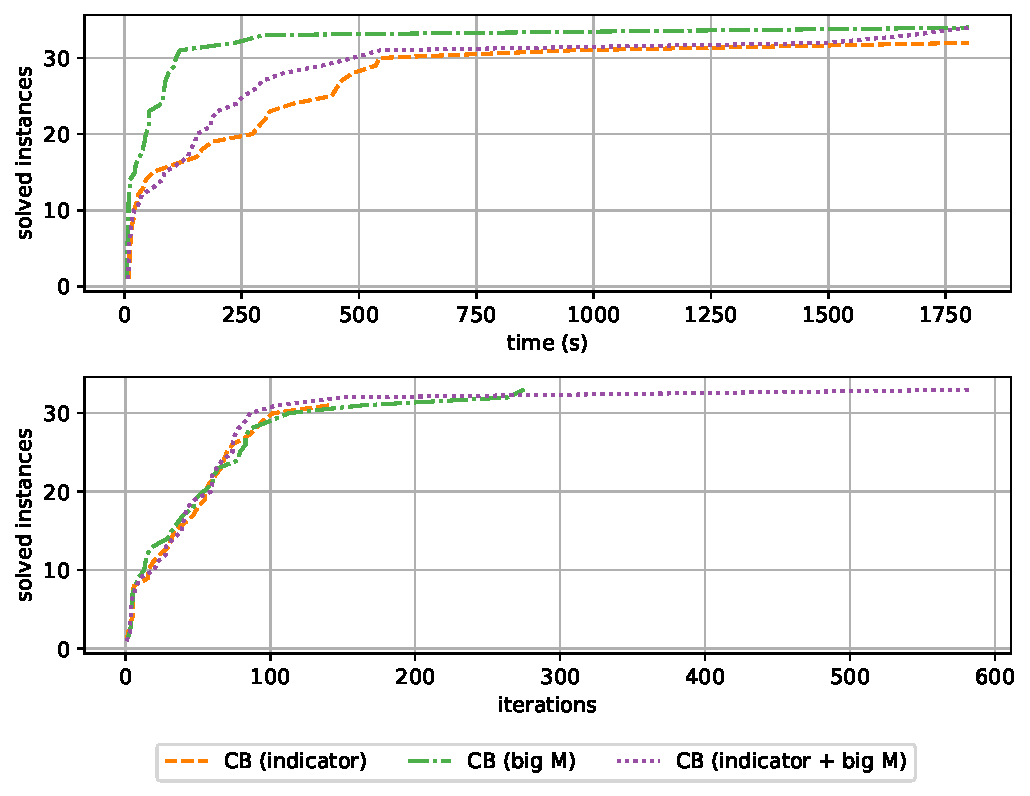
\includegraphics[width=0.8\textwidth]{Images/comparison_solved_instances_indicator_and_big_m.pdf}
    \label{fig:comparison_solved_instances_indicator_and_big_m_as_MP}
\end{figure}
\todo[inline]{add less cuts}

\begin{figure}[h!]
    \caption{solved gecko instances by CB (big M), CB (indicator) and CB (indicator and big M)}
    \centering
    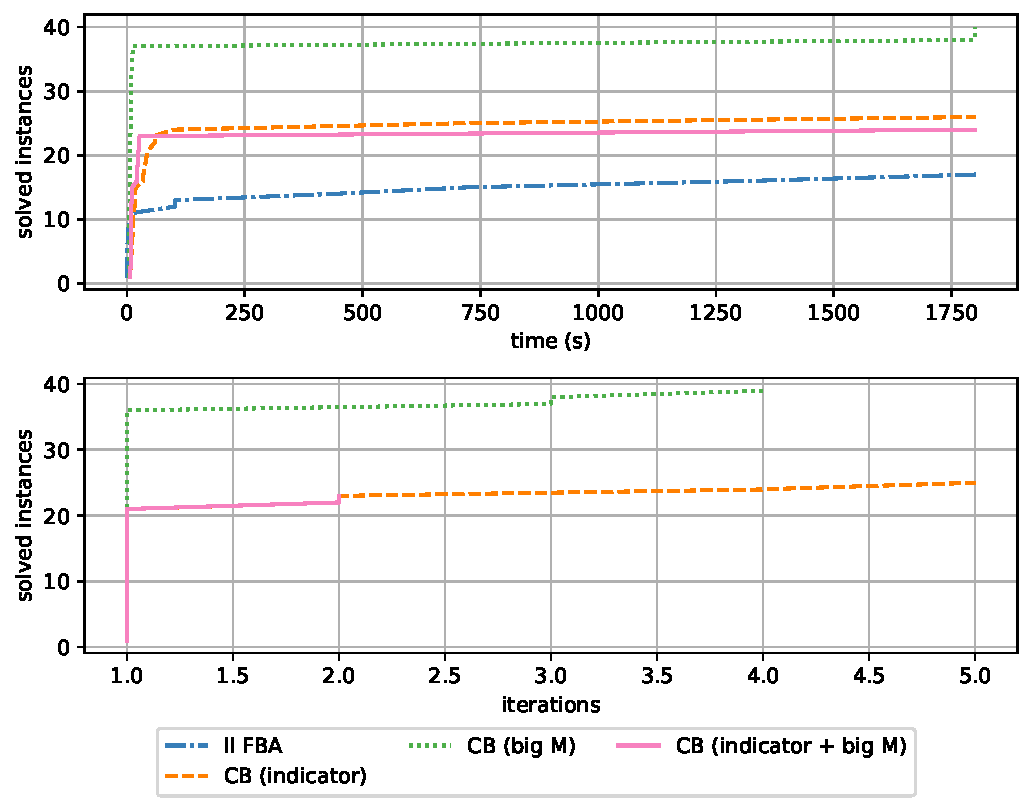
\includegraphics[width=0.8\textwidth]{Images/comparison_solved_instances_gecko_1.0e-8_indicator_and_big_m.pdf}
    \label{fig:comparison_solved_instances_gecko_1.0e-8_indicator_and_big_m_as_MP}
\end{figure}


%%%%%%%%%%%%%%%%%%%%%%%%%%%%
%%%%%Ende des Dokuments%%%%%
%%%%%%%%%%%%%%%%%%%%%%%%%%%%
\newpage
\restoreapp